\documentclass{standalone}

\begin{document}

L'objectif d'un \emph{Variational Autoencoder} est d'apprendre un encoder et un decoder comme dans un autoencoder usuel à la différence près que l'encoder du VAE va apprendre les paramètres d'une distribution de probabilité (une loi normale de paramètres $\mu, \sigma$) et que lors de l'entraînement on échantillonne cette distribution à l'entrée du decoder. Cela permet d'avoir un générateur d'échantillons décodés à partir d'un bruit gaussien passé en entrée du decoder (voir figure~\ref{vae:samples}).

\begin{figure}[H]
	\center
	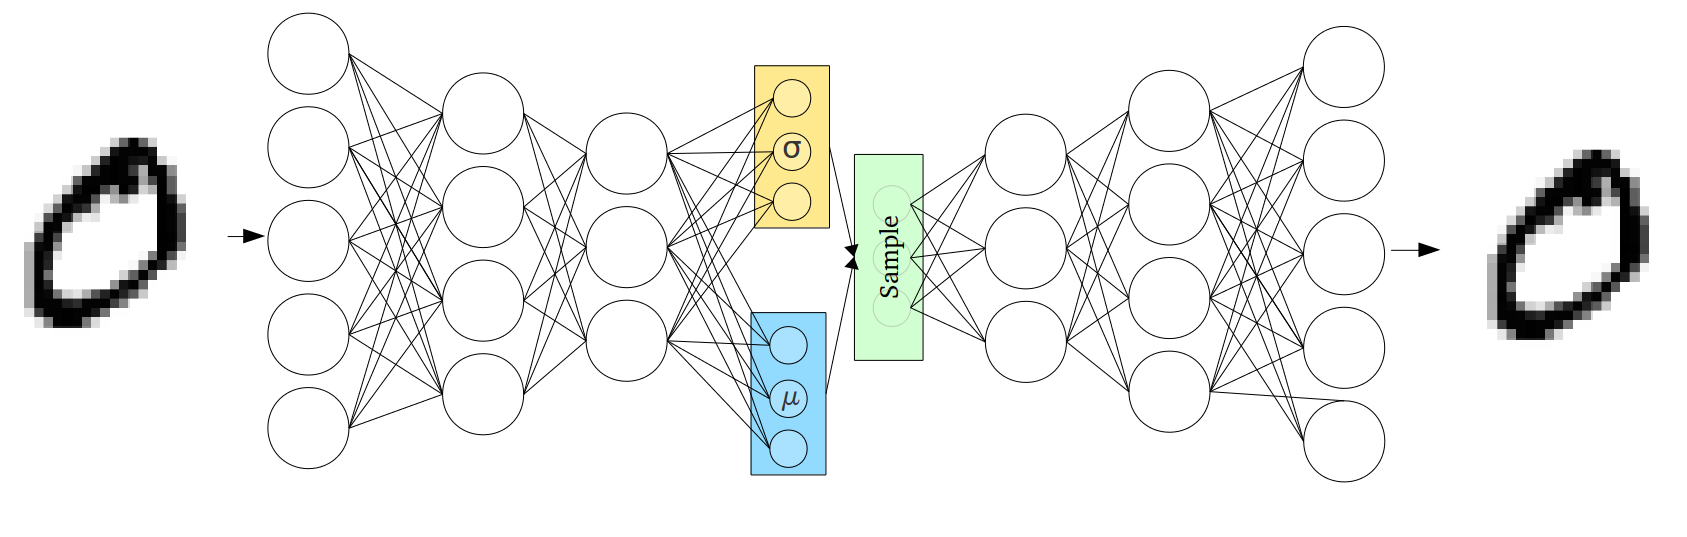
\includegraphics[scale=0.2]{img/vae.png}
	\caption{Schéma d'un VAE}
\end{figure}

\begin{figure}[ht!]
	\center
	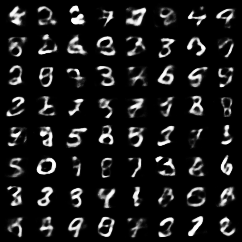
\includegraphics[scale=0.5]{img/vae_sample_10.png}
	\caption{Exemples d'échantillons produits par le decoder à partir d'un bruit Gaussien}
	\label{vae:samples}
\end{figure}

\begin{figure}[H]
	\center
	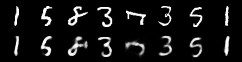
\includegraphics[scale=0.5]{img/vae_reconstruction_10.png}
	\caption{Comparaison de la reconstruction avec les entrées}
	\label{vae:reconst}
\end{figure}



\begin{minted}{python}

\end{minted}

\end{document}
